\section{Simulation-Based Inference} \label{sec:sbi}
% standard bayesian approach and introducing SBI
The ultimate goal of Bayesian SED modeling is to infer the posterior
probability distributions of galaxy properties, $\theta$, given observations,
$\xobs$  --- $p(\theta\given\xobs)$.
We can evaluate the posterior at a specific $\theta$ and ${\bf x}$ using
Bayes' rule, $p(\theta\given\xobs) \propto p(\theta)~p(\xobs\given\theta)$. 
$p(\theta)$ is the prior distribution, which we specify. 
And $p(\xobs\given\theta)$ is the likelihood, which is {\em typically}
evaluated using a Gaussian functional form: 
\beq
    \ln p(\xobs\given\theta) = -\frac{1}{2}(\xobs - m(\theta))^t {\bf C}^{-1}
    (\xobs - m(\theta)).
\eeq
$m(\theta)$ is the theoretical model, in our case a galaxy SED model from
stellar population synthesis.
${\bf C}$ is the covariance matrix of the observations. 
In practice, off-diagonal terms are often ignored and measured are
uncertainties are used as estimates of the diagonal terms. 

In the standard approach, the full posterior distribution is derived by
evaluating the posterior with a sampling technique such as Markov Chain Monte
Carlo (MCMC) or nested sampling~\citep[\eg][]{carnall2017, leja2019b,
tacchella2021}.
These sampling techniques are essential for the efficient exploration of
the relatively higher dimensionality of SED model parameter space.
Even advanced techniques, however, are subject to major limitations.  
For instance, MCMC sampling techniques can struggle to accurately estimate
multimodal and degenerate posteriors. 
Many also require significant hand-tuning by the user.
More importantly, despite their efficiency, these techniques require {\em
several million} SED model evaluations to derive a posterior --- this can
take ${\sim}100$ of CPU hours per galaxy.
Analyzing the tens of millions of spectra or billions of photometry from
upcoming surveys (\eg~DESI, Rubin, Roman) with these approaches would thus
require {\em billions of CPU hours}.

% overview of SBI and mention of ABC
A more scalable approach is available for Bayesian SED modeling:
simulation-based inference (SBI; also known as ``likelihood-free'' inference).
At its core, SBI involves any method that uses a forward model of the observed
data to directly estimate the posterior ($p(\theta\given\xobs)$), the
likelihood ($p({\bf x}\given \theta$), or the joint distribution of the
parameters and data ($p(\theta, {\bf x})$). 
SBI methods have already been successfully applied to a number of Bayesian
parameter inference problems in astronomy~\citep{cameron2012, weyant2013,
hahn2017b, kacprzak2018, alsing2018, lange2020}.
New SBI methods, such as density estimation SBI~\citep[\eg][]{papmakario2017,
alsing2018, hahn2019c},

%Density estimation likelihood-free inference works by learn- ing a parameterized model for the joint density P(θ, d), from a set of samples drawn from that density (Papamakarios & Murray 2016). In its simplest form, we start by generating a set of samples {θ, d} from P(θ, d) by drawing parameters from the prior and forward simulating mock data:
%θ ← P(θ)
%d ← P(d|θ). (4)
%We then write down a model for the joint density P(θ, d; η), parameterized by η, and fit this model to the samples {θ, d}. The estimated2 posterior density and Bayesian evidence can then be easily extracted from the fit to the joint density as follows:
%Pˆ(θ|do) ∝ P(θ,d = do;η)
%Pˆ(do) =
%∫
%P(θ, d = do; η) dθ, (5)
%ie., taking a slice through the joint distribution evaluated at the observed data d = do, and subsequently integrating over the parameters for the Bayesian evidence. For many prac- tical choices of parameterized models for the joint density, eg., Gaussian mixture models (see below), the evidence in- tegral in Eq. (5) is analytically tractable. This means that the evidence comes for free, and if the parameterized model for the joint density is fit to the samples in a principled way, the uncertainties on the fit parameters can be propa- gated through to a principled uncertainty on the estimated Bayesian evidence.
%In contrast to abc, delfi uses all of the available for- ward simulations {θ,d} to inform the inference of the joint density P(θ, d), and hence the posterior density and evidence estimation. In practice, this means that far fewer forward simulations may be needed to obtain high-fidelity posterior inferences (compared to abc that has a vanishingly small ac- ceptance rate as ε → 0), as demonstrated by Papamakarios & Murray (2016).




%In one popular SBI method, Approximate Bayesian Computation (ABC), a rejection
%sampling framework is used to estimate the posterior. 
%First, parameter values are sampled from the prior: $\theta'\sim p(\theta)$. 
%For each sampled $\theta'$, the forward model is run then compared to the
%observed data, ${\bf x}$. 
%If the forward model reproduces ${\bf x}$, $\theta'$ is kept; otherwise, it is
%rejected. 
%This process is repeated until there are enough samples to estimate the
%posterior. 


\subsection{Amortized Neural Posterior Estimation} \label{sec:flow}
% section explaining conditional normalizing flows and how we condition on the
% noise itself


\begin{figure}
\begin{center}
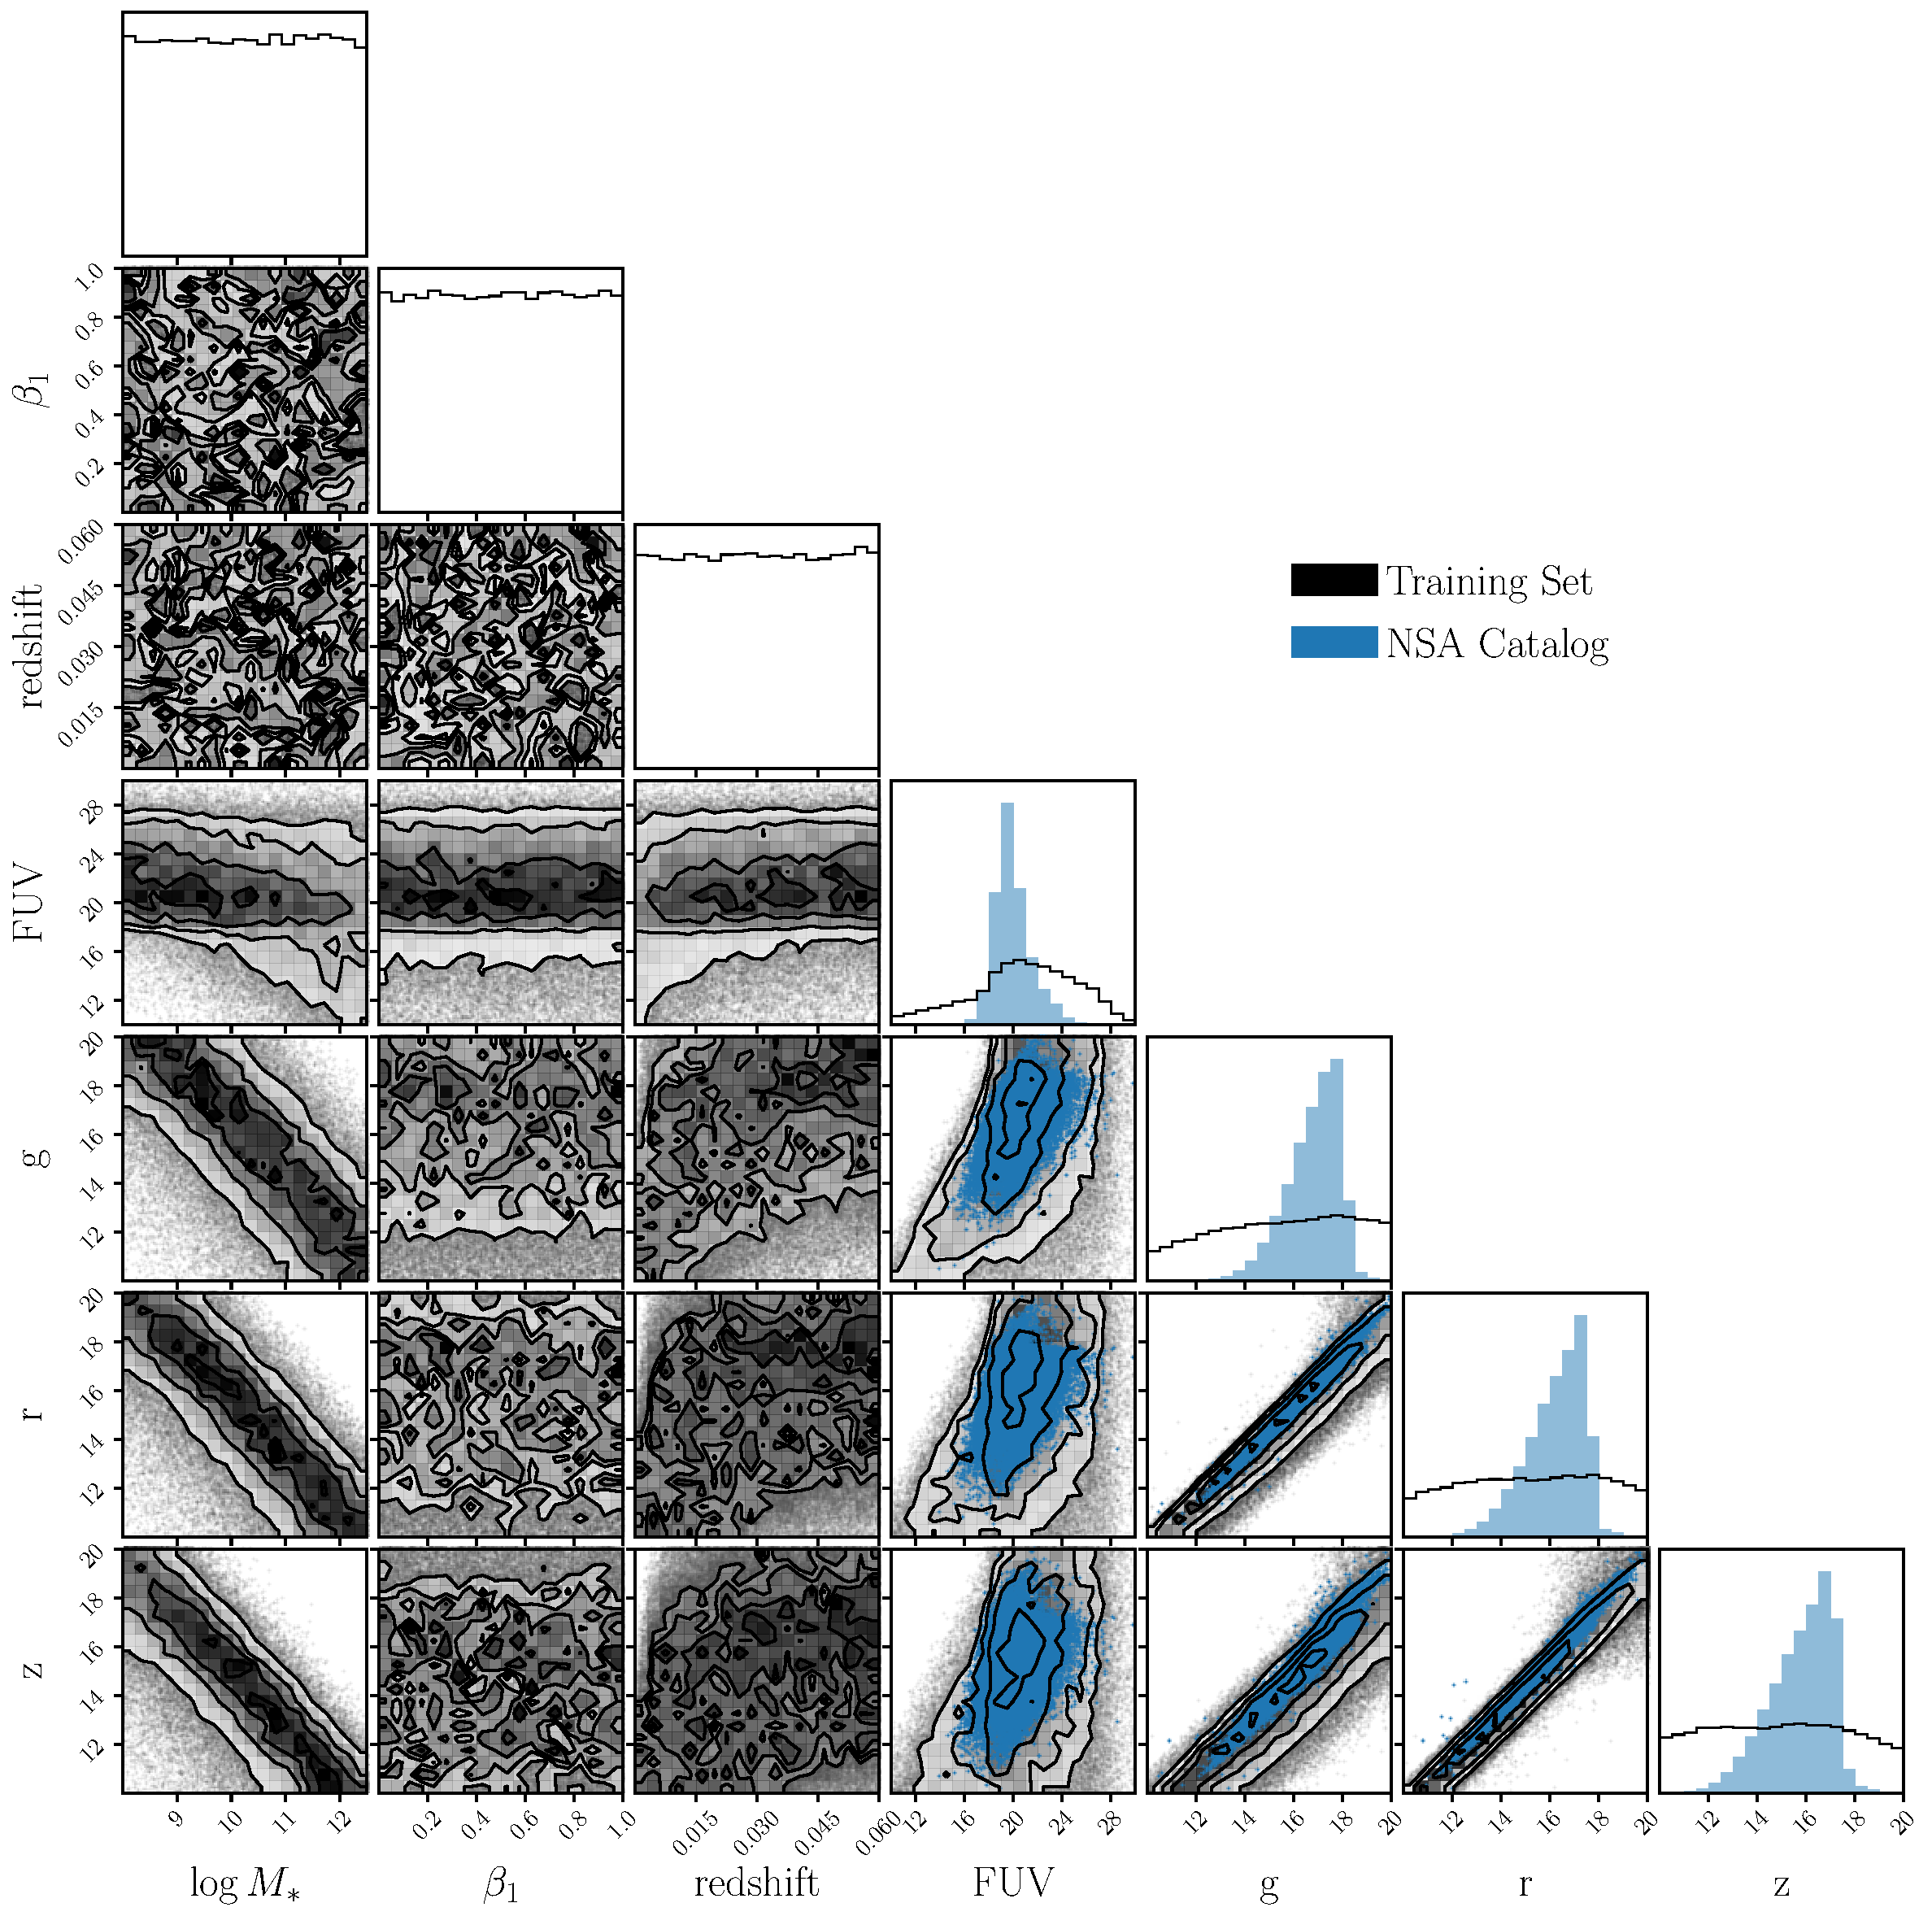
\includegraphics[width=0.9\textwidth]{figs/sbi.pdf}
    \caption{\label{fig:sbi}
    Joint distribution of SED model parameters ($\log M_*$, $\beta_1$,
    redshift) and photometric magnitudes (FUV, $g$, $r$, $z$) for our training
    set. 
    The training set was constructed by sampling parameter values from the
    prior (Table~\ref{tab:prior}), constructing SEDs using a theoretical SPS
    model, and applying our noise model. 
    For details, we refer readers to Section~\ref{sec:sbi_sed}.
    For comparison, we present the distribution of magnitudes for galaxies in
    the NSA catalog (blue). 
    \emph{The training set fully encompasses the observations, thus, our 
    {\sc SEDflow} method can be used to infer the posterior for all NSA
    galaxies}.
    }
\end{center}
\end{figure}


